\documentclass{article}
\usepackage{../../mypackages}
\usepackage{../../macros}

% Variable de correction


% Variable de correction
% \newif\ifWITHCORRECTION
% \WITHCORRECTIONtrue % Mettre \WITHCORRECTIONfalse pour la version élève

% Commandes pour masquer du texte en fonction de la version
%\newcommand{\corrige}[2]{\ifWITHCORRECTION #1 \else \underline{\hspace{#2}} \fi}


\def\WITH_CORRECTION{YES}

\title{Chapitre 2 - Les Matériaux Organiques}
\author{N. Bancel}
\date{Septembre 2024}

\renewcommand{\arraystretch}{2} % Increases row height by 2x

\begin{document}

\maketitle

% Rappels de 2nde
\section{Rappels de 2nde}

\subsection{Couches électroniques et électrons de valence}

\begin{tcolorbox}[colback=green!10!white, colframe=green!75!black, title=Définitions : ]
  Les électrons se répartissent autour du noyau atomique selon des couches électroniques et des sous-couches. \par 
  \vspace{1em}
  Les \textbf{couches électroniques} sont notées \(n = 1, 2, 3\) etc \par 
  Chaque couche électronique est divisée en \textbf{sous-couches} qui sont notées par les lettres \(s\), \(p\), etc.
  \begin{itemize}[noitemsep]
    \item La sous-couche \(s\) peut contenir jusqu'à 2 électrons.
    \item La sous-couche \(p\) peut contenir jusqu'à 6 électrons.
  \end{itemize}

  Dans la configuration électronique à l'état fondamental d'un atome de numéro atomique inférieur ou égal à 18, les électrons \textit{ns} et \textit{np} associés à la plus grande valeur de \textit{n} sont appelés \textbf{électrons de valence}
  
  Seuls les électrons de la couche externe (électrons de valence) participent aux liaisons entres atomes dans les molécules, ou à la formation d’ions. 
  
\end{tcolorbox}

\begin{tcolorbox}[colback=blue!10!white, colframe=blue!75!black, title=Application : Structure électronique]
  Exemple de l'atome d'oxygène (O) : Numéro atomique : \(Z = 8\) \\
  Sa configuration électronique est : \(1s^2 2s^2 2p^4\). \\
  Cela signifie :
  \begin{itemize}[noitemsep]
    \item 2 électrons dans la première couche (1s$^2$)
    \item 2 électrons dans la sous-couche s de la deuxième couche (2s$^2$)
    \item 4 électrons dans la sous-couche p de la deuxième couche (2p$^4$)
  \end{itemize}
  Il possède donc 6 électrons de valence (2s$^2$ 2p$^4$).
\end{tcolorbox}

\vspace{1em}


\subsection{Stabilité}

\begin{tcolorbox}[colback=red!10!white, colframe=red!75!black, title=Important]
\textbf{Règle de stabilité} : au cours des transformations chimiques, les atomes acquièrent la même configuration électronique que celle d'un atome de gaz noble, c'est-à-dire une configuration électronique de valence en duet ou en octet. \par
\vspace{1em}
Ils cherchent à obtenir une couche de valence \textbf{remplie}. Composée donc de soit 2 électrons, soit 8 électrons
\end{tcolorbox}

\begin{tabularx}{\linewidth}{|| p{2cm} | p{1.5cm} | X | p{3cm} | X ||}
  \toprule
  {Atome} & {Numéro atomique} & {Configuration électronique} & {\# électrons nécessaires pour remplir la couche de valence ?} & {Gaz noble ?} \\
  \midrule
  {Hélium (\ce{He})} & {2} & {} & {} \\ 
  {Carbone (\ce{C})} & {14} & {} & {} \\ 
  {Néon (\ce{Ne})} & {10} & {} & {} \\
  {Oxygène (\ce{O})} & {16} & {} & {} \\ 
  {Argon (\ce{Ar})} & {18} & {} & {} \\
  {Azote (\ce{N})} & {15} & {} & {} \\ 
  {Hydrogène (\ce{H})} & {1} & {} & {} \\
  {Chlore (\ce{Cl})} & {17} & {} & {} \\ 
  \bottomrule
\end{tabularx}


\subsection{Stabilité chimique et liaisons chimiques}

\subsubsection{Couche de valence}

\begin{figure}[H]
  \centering
  \includegraphics[width=\linewidth]{stabilité_chimique.jpg}
  \caption{\label{} Stabilité chimique}
\end{figure}



\begin{tcolorbox}[colback=green!10!white, colframe=green!75!black, title=Définitions : ]
  Dans une molécule, les atomes mettent des électrons de valence en commun avec d’autres atomes afin d’obtenir la configuration électronique de valence en duet ou en octet. \par
  \vspace{1em}
  La mise en commun de deux électrons de valence par deux atomes permet la réalisation d’une liaison chimique.
  \vspace{1em}
  Plus familièrement : \textit{"Si je prends un électron, j'en donne un"}
\end{tcolorbox}

\subsubsection{Les doublets liants / non liants}

Dans une molécule, les atomes possèdent sur leur couche électronique de valence deux types de doublets électroniques (paquet de deux électrons).
\begin{itemize}[noitemsep]
  \item Les doublets liants constituent les liaisons chimiques réalisées avec d’autres atomes.
  \item Les doublets non liants appartiennent uniquement à l’atome
\end{itemize}

\subsubsection{Les doublets liants / non liants}

\begin{figure}[H]
  \centering
  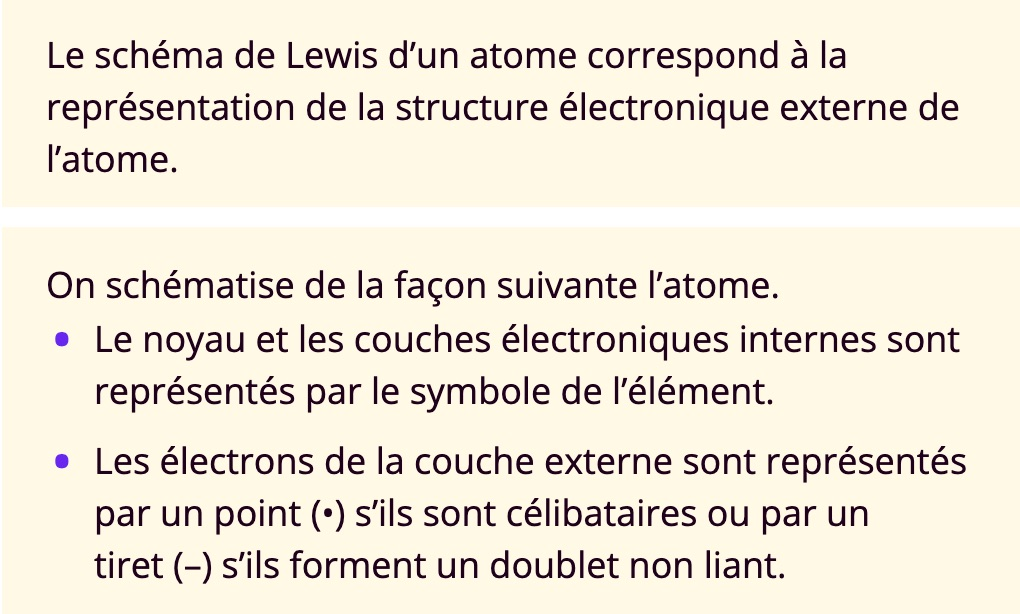
\includegraphics[width=0.6\linewidth]{lewis.jpg}
  \caption{\label{} Schéma de Lewis}
\end{figure}


\begin{tabular}{|| p{3cm} | p{6cm} | p{4cm} ||}
  \toprule
  {Atome} & {Nombres d'électrons "célibataires" / ayant besoin de se lier avec l'électron d'un autre atome} & {Schéma de Lewis} \\
  \midrule
  {Hydrogène (\ce{H})} & {} & {} \\
  {Carbone (\ce{C})} & {} & {} \\ 
  {Azote (\ce{N})} & {} & {} \\ 
  {Oxygène (\ce{O})} & {} & {} \\ 
  {Chlore (\ce{Cl})} & {} & {} \\ 
  \bottomrule
\end{tabular}

\subsubsection{Exemples d'application + Représenttion des molécules}

Le schéma de Lewis d’une molécule correspond à la représentation des atomes qui constituent la molécule et de leurs doublets liants et non liants. \par
\vspace{1em}
On représente un doublet liant par un tiret entre les deux atomes liés, et un doublet non liant par un tiret à côté de l’atome. \par
\vspace{1em}
En s'aidant des tableaux remplis au-dessus, et du cours, dessiner le schéma de Lewis des molécules suivantes 

\begin{itemize}[noitemsep]
  \item Eau : \ce{H2O}
  \item Méthane : \ce{CH4}
  \item Ammoniac : \ce{NH3}
  \item Dioxygène : \ce{O2}
  \item Dioxyde de carbone : \ce{CO2}
\end{itemize}

Réponses : 

\vspace{7em}


\section{Les chaînes carbonées}

\subsection{L'atome de carbone}

\begin{figure}[H]
  \centering
  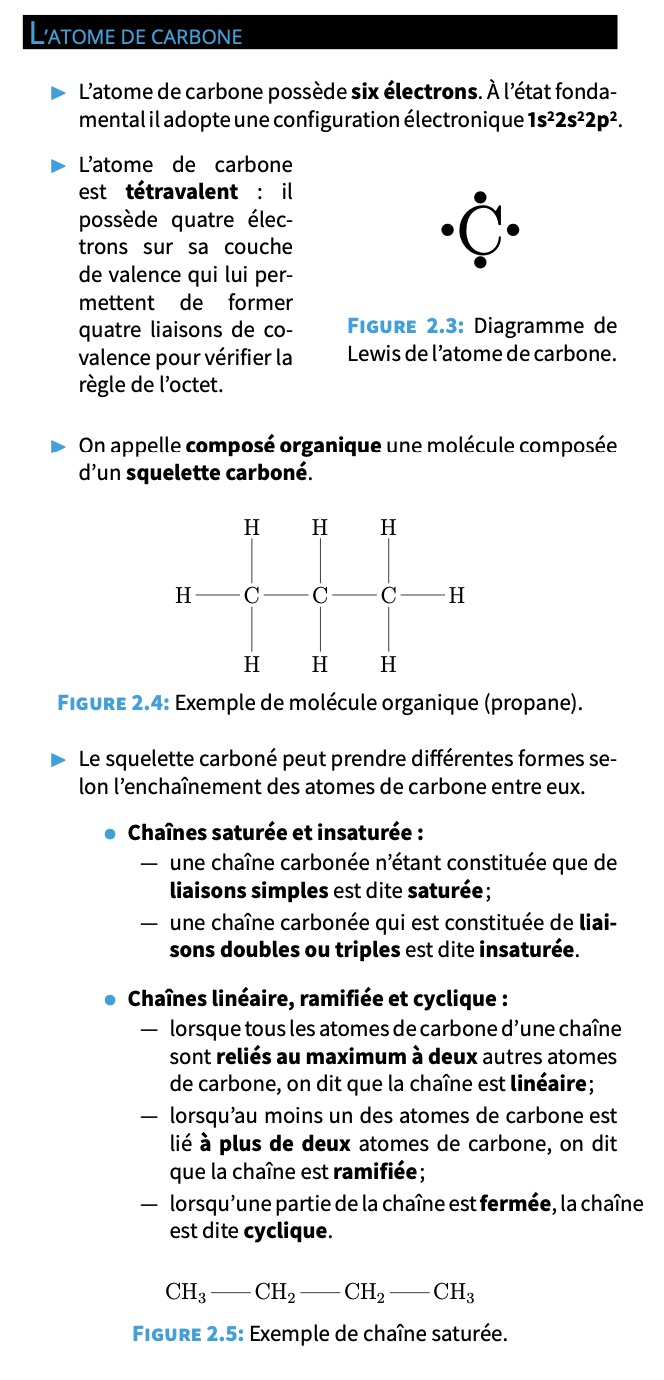
\includegraphics[width=0.6\linewidth]{livre_page1.jpg}
  \caption{\label{} Chaînes carbonées}
\end{figure}

\subsection{Modélisation de molécules}

\begin{figure}[H]
  \centering
  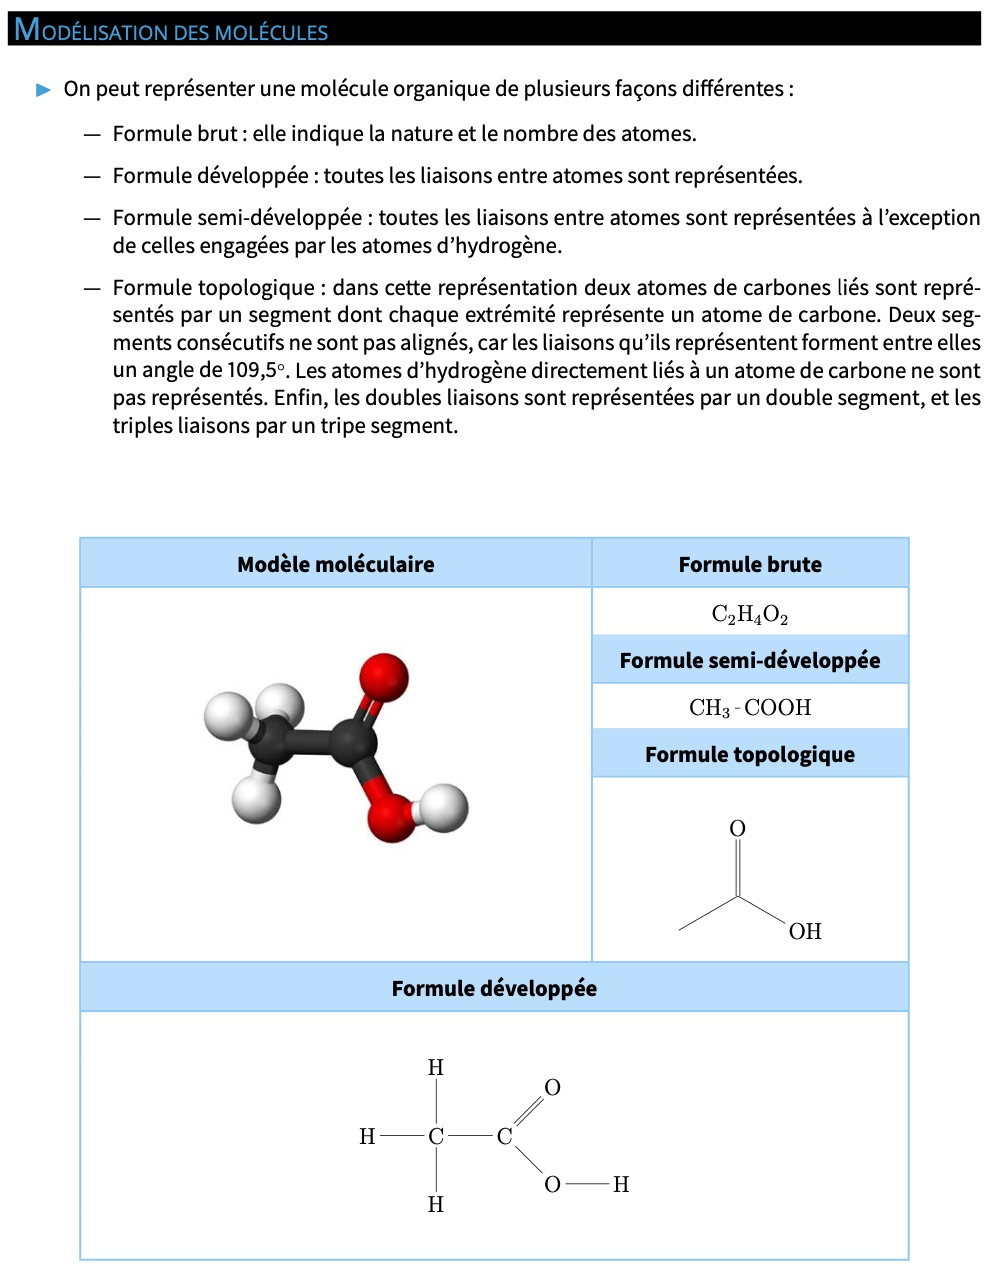
\includegraphics[width=0.6\linewidth]{livre_page2.jpg}
  \caption{\label{} Modélisation de molécules}
\end{figure}

\subsection{Mise en application}

\begin{tcolorbox}[colback=blue!10!white, colframe=blue!75!black, title=Application : Structure électronique]
  Exercices à faire en groupe (dans le livre de Physique) : 
  \begin{itemize}[noitemsep]
    \item N°1
    \item N°2
    \item N°3 page 40
  \end{itemize}
\end{tcolorbox}





\section{Sources}

Quelques cours / sources intéressantes : 

\begin{itemize}[noitemsep]
  \item \href{https://www.maxicours.com/se/cours/etablir-le-schema-de-lewis-et-la-geometrie-d-une-molecule/}{Maxicours}
  \item \href{https://www.youtube.com/watch?v=bmV-Tbv2Me8&ab_channel=e-profs-PhysiqueChimie}{Vidéo Youtube}
\end{itemize}



\end{document}
